%%
%% This is file `sample-sigplan.tex',
%% generated with the docstrip utility.
%%
%% The original source files were:
%%
%% samples.dtx  (with options: `sigplan')
%% 
%% IMPORTANT NOTICE:
%% 
%% For the copyright see the source file.
%% 
%% Any modified versions of this file must be renamed
%% with new filenames distinct from sample-sigplan.tex.
%% 
%% For distribution of the original source see the terms
%% for copying and modification in the file samples.dtx.
%% 
%% This generated file may be distributed as long as the
%% original source files, as listed above, are part of the
%% same distribution. (The sources need not necessarily be
%% in the same archive or directory.)
%%
%% The first command in your LaTeX source must be the \documentclass command.
\documentclass[sigplan,screen]{acmart}
\usepackage{subcaption}
\usepackage{todonotes}
\usepackage{xcolor}
\usepackage{amsmath}
\usepackage{bm}
\usepackage{algorithm}
\usepackage{algcompatible}
%% NOTE that a single column version is required for 
%% submission and peer review. This can be done by changing
%% the \doucmentclass[...]{acmart} in this template to 
%% \documentclass[manuscript,screen,review]{acmart}
%% 
%% To ensure 100% compatibility, please check the white list of
%% approved LaTeX packages to be used with the Master Article Template at
%% https://www.acm.org/publications/taps/whitelist-of-latex-packages 
%% before creating your document. The white list page provides 
%% information on how to submit additional LaTeX packages for 
%% review and adoption.
%% Fonts used in the template cannot be substituted; margin 
%% adjustments are not allowed.
%%
%% \BibTeX command to typeset BibTeX logo in the docs
\AtBeginDocument{%
  \providecommand\BibTeX{{%
    \normalfont B\kern-0.5em{\scshape i\kern-0.25em b}\kern-0.8em\TeX}}}

%% Rights management information.  This information is sent to you
%% when you complete the rights form.  These commands have SAMPLE
%% values in them; it is your responsibility as an author to replace
%% the commands and values with those provided to you when you
%% complete the rights form.
\setcopyright{acmcopyright}
\copyrightyear{2022}
\acmYear{2022}
\acmDOI{XXXXXXX.XXXXXXX}

%% These commands are for a PROCEEDINGS abstract or paper.
\acmConference[SC '22]{Make sure to enter the correct
  conference title from your rights confirmation emai}{Novemeber 13--18,
  2022}{Dallas, Texas, USA}
%
%  Uncomment \acmBooktitle if th title of the proceedings is different
%  from ``Proceedings of ...''!
%
%\acmBooktitle{Woodstock '18: ACM Symposium on Neural Gaze Detection,
%  June 03--05, 2018, Woodstock, NY} 
\acmPrice{15.00}
\acmISBN{978-1-4503-XXXX-X/18/06}


%%
%% Submission ID.
%% Use this when submitting an article to a sponsored event. You'll
%% receive a unique submission ID from the organizers
%% of the event, and this ID should be used as the parameter to this command.
%%\acmSubmissionID{123-A56-BU3}

%%
%% The majority of ACM publications use numbered citations and
%% references.  The command \citestyle{authoryear} switches to the
%% "author year" style.
%%
%% If you are preparing content for an event
%% sponsored by ACM SIGGRAPH, you must use the "author year" style of
%% citations and references.
%% Uncommenting
%% the next command will enable that style.
%%\citestyle{acmauthoryear}

%%
%% end of the preamble, start of the body of the document source.
\begin{document}

%%
%% The "title" command has an optional parameter,
%% allowing the author to define a "short title" to be used in page headers.
\title[Reinforcement learning approach for mapping applications to dataflow-based CGRA]{Reinforcement learning approach for mapping applications to dataflow-based Coarse-Grained Reconfigurable Array}

%%
%% The "author" command and its associated commands are used to define
%% the authors and their affiliations.
%% Of note is the shared affiliation of the first two authors, and the
%% "authornote" and "authornotemark" commands
%% used to denote shared contribution to the research.
% \author{Parth}
% \authornote{Both authors contributed equally to this research.}
% \email{trovato@corporation.com}
% \orcid{1234-5678-9012}
% \author{G.K.M. Tobin}
% \authornotemark[1]
% \email{webmaster@marysville-ohio.com}
% \affiliation{%
%   \institution{Institute for Clarity in Documentation}
%   \streetaddress{P.O. Box 1212}
%   \city{Dublin}
%   \state{Ohio}
%   \country{USA}
%   \postcode{43017-6221}
% }

% \author{Andre Chang}
% \affiliation{%
%   \institution{The Th{\o}rv{\"a}ld Group}
%   \streetaddress{1 Th{\o}rv{\"a}ld Circle}
%   \city{Hekla}
%   \country{Iceland}}
% \email{larst@affiliation.org}

% \author{Valerie B\'eranger}
% \affiliation{%
%   \institution{Inria Paris-Rocquencourt}
%   \city{Rocquencourt}
%   \country{France}
% }

% \author{Abhishek Chaurasia}
% \affiliation{%
%  \institution{Rajiv Gandhi University}
%  \streetaddress{Rono-Hills}
%  \city{Doimukh}
%  \state{Arunachal Pradesh}
%  \country{India}}

% \author{Huifen Chan}
% \affiliation{%
%   \institution{Tsinghua University}
%   \streetaddress{30 Shuangqing Rd}
%   \city{Haidian Qu}
%   \state{Beijing Shi}
%   \country{China}}

% \author{Charles Palmer}
% \affiliation{%
%   \institution{Palmer Research Laboratories}
%   \streetaddress{8600 Datapoint Drive}
%   \city{San Antonio}
%   \state{Texas}
%   \country{USA}
%   \postcode{78229}}
% \email{cpalmer@prl.com}

% \author{John Smith}
% \affiliation{%
%   \institution{The Th{\o}rv{\"a}ld Group}
%   \streetaddress{1 Th{\o}rv{\"a}ld Circle}
%   \city{Hekla}
%   \country{Iceland}}
% \email{jsmith@affiliation.org}

% \author{Julius P. Kumquat}
% \affiliation{%
%   \institution{The Kumquat Consortium}
%   \city{New York}
%   \country{USA}}
% \email{jpkumquat@consortium.net}

%%
%% By default, the full list of authors will be used in the page
%% headers. Often, this list is too long, and will overlap
%% other information printed in the page headers. This command allows
%% the author to define a more concise list
%% of authors' names for this purpose.
% \renewcommand{\shortauthors}{Trovato and Tobin, et al.}

%%
%% The abstract is a short summary of the work to be presented in the
%% article.
\begin{abstract}
The Streaming Engine (SE) is a Coarse-Grained Reconfigurable Array developed by Micron 
Technology.
The SE provides programming flexibility and high-performance with energy efficiency.
%A program is broken down into a set of one or more Synchronous Data-Flows (SDFs).
A program is represented as a computation graph, where every instruction is a node.
Each node needs to be mapped to the right slot and array in the SE to ensure the correct execution of the program.
This creates an optimization problem with a vast and sparse search space.
A manual mapping of the graph takes an infeasible amount of time by the programmer.
Such manual mapping is impractical because it requires expertise and knowledge in the SE micro-architecture and reduces the search-space, thus, trading off optimization possibilities.
In this work we propose a Reinforcement Learning(RL) based mapper to explore mappings and optimize them in an unsupervised manner using a reinforcement learning framework.
This provides us an automated method that can produce mappings for programs quickly and searches for optimal mappings without programmers interference. 
This tool also improves the usability of the SE device by encapsulating device configuration details.
We use Proximal Policy Optimization (PPO) in order to train a model which places operations into the SE tiles based on a reward function that models the SE device and its constraints.
Graph neural networks are added to create embeddings to represent the computation graph.
A transformer block is used to model sequential operation placement mode. 
We show results on how certain workloads are mapped to the SE.
% The implemented method is compared against evolutionary search and baseline.
\end{abstract}

%%
%% The code below is generated by the tool at http://dl.acm.org/ccs.cfm.
%% Please copy and paste the code instead of the example below.
%%
\begin{CCSXML}
<ccs2012>
 <concept>
  <concept_id>10010520.10010553.10010562</concept_id>
  <concept_desc>Computer systems organization~Embedded systems</concept_desc>
  <concept_significance>500</concept_significance>
 </concept>
 <concept>
  <concept_id>10010520.10010575.10010755</concept_id>
  <concept_desc>Computer systems organization~Redundancy</concept_desc>
  <concept_significance>300</concept_significance>
 </concept>
 <concept>
  <concept_id>10010520.10010553.10010554</concept_id>
  <concept_desc>Computer systems organization~Robotics</concept_desc>
  <concept_significance>100</concept_significance>
 </concept>
 <concept>
  <concept_id>10003033.10003083.10003095</concept_id>
  <concept_desc>Networks~Network reliability</concept_desc>
  <concept_significance>100</concept_significance>
 </concept>
</ccs2012>
\end{CCSXML}

\ccsdesc[500]{Computer systems organization~Embedded systems}
\ccsdesc[300]{Computer systems organization~Redundancy}
\ccsdesc{Computer systems organization~Robotics}
\ccsdesc[100]{Networks~Network reliability}

%%
%% Keywords. The author(s) should pick words that accurately describe
%% the work being presented. Separate the keywords with commas.
\keywords{reinforcement learning, data-flow mapping, coarse grain reconfigurable array}

%% A "teaser" image appears between the author and affiliation
%% information and the body of the document, and typically spans the
%% page.
% \begin{teaserfigure}
%   \includegraphics[width=\textwidth]{sampleteaser}
%   \caption{Seattle Mariners at Spring Training, 2010.}
%   \Description{Enjoying the baseball game from the third-base
%   seats. Ichiro Suzuki preparing to bat.}
%   \label{fig:teaser}
% \end{teaserfigure}

%%
%% This command processes the author and affiliation and title
%% information and builds the first part of the formatted document.
\maketitle

\section{Introduction}
\label{sec:intro}
As Dennard scaling ends, big-data applications such as real-time image processing, graph analytics, and deep learning continue to push the boundaries of performance and energy efficiency requirements for computing system. 
One solution to this challenge is to move compute closer to memory or storage for substantial energy savings of data movement. 
We have developed an innovative Near-Data Computing (NDC) architecture that leverages the dramatic opportunities provided by the new CXL protocol \cite{sharma2020compute}. 
NDC incorporates heterogenous compute elements in the memory/storage subsystem to accelerate various computing tasks near data. 
One of these compute elements is the Streaming Engine (SE).

The SE is a Coarse-Grained Reconfigurable Array (CGRA) that is composed of interconnected compute tiles.  
The compute tiles are interconnected with both a Synchronous Fabric (SF) and an Asynchronous Fabric (AF) as shown in Fig. \ref{fig:sub-se}.
It also interconnects tile memory, multiplexers, and Single Instruction Multiple Data (SIMD) units within each tile as shown in Fig. \ref{fig:sub-tile}. 
Tiles can be pipelined through SF to form a Synchronous Data Flow (SDF) through Multiply/Shift (MS) unit and an Arithmetic/Logic (AL) SIMD units. 
The output of the MS unit is connected to one of the two inputs of the AL unit.
AF connects a tile with all other tiles, dispatch interface (DI), and memory interfaces (MI).
It bridges SDFs through asynchronous operations, which include SDF initiation, asynchronous data transfer from one SDF to another, system memory accesses, and branching and looping constructs. 
Together, SF and AF allow the tiles to efficiently execute high-level programming language constructs.
Simulation results of hand-crafted SE kernels have shown orders-of-magnitude better performance per watt on data-intensive applications than existing computing platforms.

\begin{figure}
  \centering
  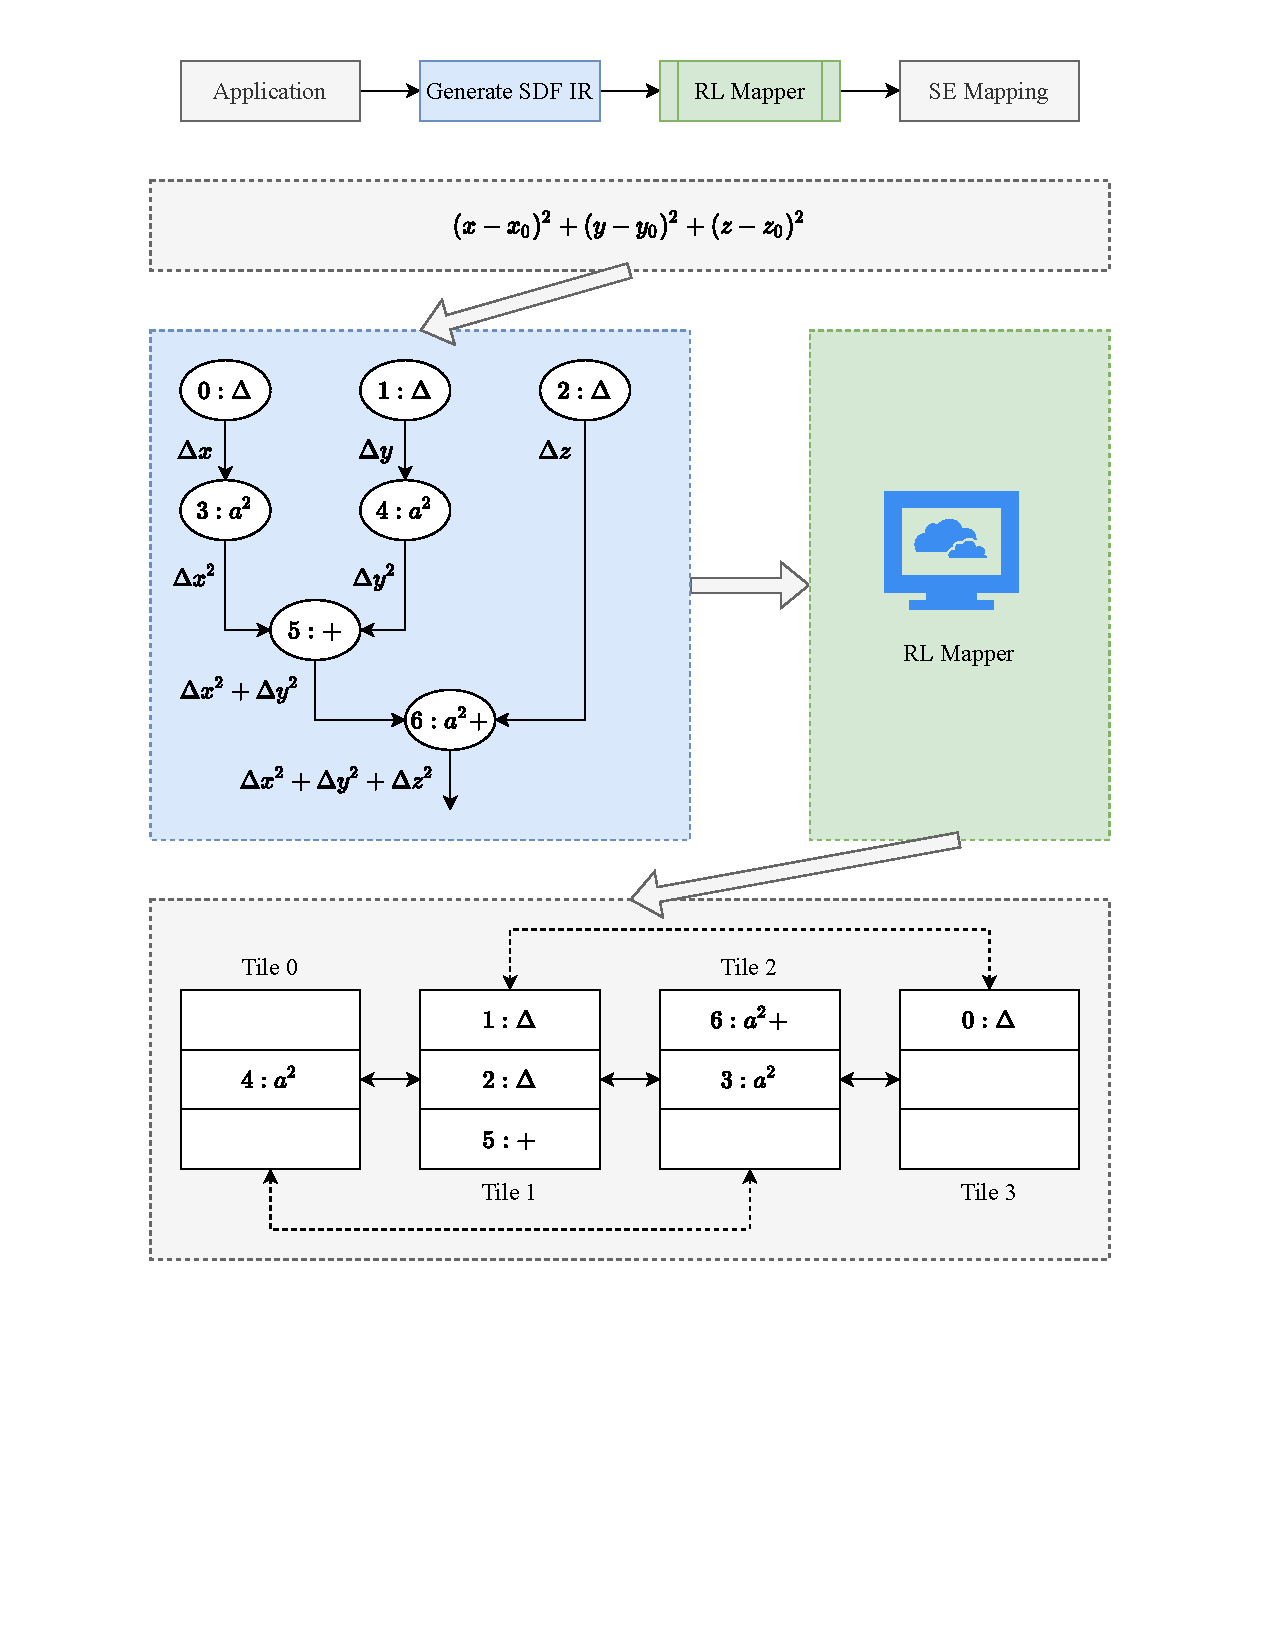
\includegraphics[trim=70 180 70 25, clip, width=\linewidth]{fig/SE_example.pdf}
  \caption{
    Example showing a mapping of a distance calculation function onto the SE device.
    The instruction execution latency is three clock cycles.
    The solid and dotted lines connecting the tiles, have one and two clock cycles transfer latency respectively.
    E.g., instruction \#0 is scheduled at (tile \#3, slot \#0) and its output is sent to instruction \#3.
    Instruction \#0 output is ready after three clock cycles plus two clock cycles to move data to tile \#1. 
    Thus, instruction \#3 gets scheduled on (tile \#1, slot \#1).
  }
  \label{fig:se_example}
\end{figure}

A simple example that illustrates a program mapped to the SE is shown in \figurename~\ref{fig:se_example}.
The program in this example is a distance calculation function shown in Eq. \ref{eq:dist}.

\begin{equation}
    \label{eq:dist}
    D = \sqrt{(x - x_0)^2 +(y - y_0)^2 + (z - z_0)^2}
\end{equation}

To keep this example simple, we ignore the square root part of the equation.
The program is represented as a Data-Flow Graph (DFG) as shown in \figurename~\ref{fig:se_example}.
Each operation in Eq. \ref{eq:dist} is an instruction that is mapped to a slot at a tile on the SE.

Since the output of the MS unit is connected to the input of the AL unit, instruction \#6 produces $\Delta z^2$ on the output on the MS unit and adds it to $(\Delta x^2 + \Delta y^2)$ at the AL unit.


Mapping the instructions from a program's DFG onto the compute elements of the SE while adhering to architectural constraints is an NP-hard problem with a vast and sparse search space \cite{10.1007/3-540-69346-7_30}. 
Constraints related to tile memory, synchronous dataflow, the use of delays to match timing requirements and more are necessary to ensure correct execution. 
Creating the mappings manually or using brute force algorithms takes time and lots of effort even for the simplest of programs. 
This process also adds assumptions that reduce the search space, trading off optimization possibilities.  

In this work we propose a deep Reinforcement Learning (RL) method to explore and find optimal mappings in an unsupervised manner. 
Using the Proximal Policy Optimization (PPO) method we train a neural network model to place instructions onto the SE tiles guided by a reward function in an environment that models the SE device and its constraints. 
We also present Global Graph Attention module that improves the baseline feedforward models by providing attention mechanism to the RL model.
Our RL method is combined with output masking, finetuning and sorted iteration order, which will be presented in the following sections.

The trained model is able to create valid mappings for the SE by learning about the structure of the problem domain.
On average addition of GGA finds 10\% better instruction schedules in terms of clock cycles for varying graphs complexities and different SE device configurations.

The key contributions of this paper are as follows:
\begin{enumerate}
    \item A Reinforcement Learning methodology that is able to map the instructions from a given DFG to the processing elements in the SE and has the potential to be reused across SDF graphs.
    \item An analysis of different factors that impacts the quality of mappings obtained, such as attention module, output masking and iteration order.
\end{enumerate}

This work is motivated by the need to provide an improved SE toolset that lowers the SE usability barrier for a programmer.
This will also assist other tools or programmers in SE mapping creation by providing partial placement suggestions or tile configuration labels.
The RL mapper performs unsupervised learning and optimization allowing it to search a wide and sparse search space. 
Each node in the DFG is an instruction that is mapped to a specific slot on a tile.

This line of research is inspired by recent work that used RL for chip placement \cite{mirhoseini2020chip}.
The problem requirement of mapping nodes of a DFG to available compute elements is similar to the problem of placing nodes of a chip netlist on a chip canvas. 
% Due to the similarities between these problem domains, we theorize that our approach has the potential of being used for chip placement.
% This hypothesis will be investigated in future work.

The rest of this paper is organized as follows: 
Section \ref{sec:relatedwork} discusses related work.
Section \ref{sec:background} provides the necessary background on the SE device architecture needed to understand the details of the RL approach.
Section \ref{sec:rlmapper} presents the proposed RL approach for mapping applications to the SE.
Section \ref{sec:results} discusses results, and Section \ref{sec:conclusion} concludes the paper along with a discussion on future work.

\section{Related work}
\label{sec:relatedwork}
\subsection{CGRA}
CGRAs are a heavily researched architectural paradigm with a long history and can provide an excellent balance of high-performance compute, memory bandwidth, and area and energy efficiency \cite{theodoridis2007survey}.
Due to such advantages, CGRAs are currently enjoying a resurgence in interest, not just in the research realm \cite{prabhakar2018plasticine}, but also commercially \cite{morgan2018intel, nicol2017coarse, vissers2019versal}.
Research compilers targeting CGRAs are available (for example, \cite{adriaansen2016code, chin_cgra-me_2017, mei2003exploiting, prabhakar2018plasticine}) but they are limited in quality and code coverage. 
Industry-strength compilers such as Clang/LLVM do not provide official support for CGRA-like architectures.
For further information on the various taxonomy of CGRAs architectures and design, we refer the reader to \cite{liu_survey_2019, tehre_survey_2012}.

Mapping various programming constructs onto CGRAs is an extensive research topic.
The  mapping of large and irregular loops onto CGRAs is analyzed in \cite{zhao_towards_2020} which proposed paying more attention to temporal mapping than spatial mapping. 
The proposed temporal mapping utilizes a buffer allocating heuristic with constraint on computations and interconnection resources. 
The proposed spatial mapping uses a backtracking and reordering mechanism with greedy algorithm with the goal of minimizing the Initiation Interval (II).
A method for mapping SDFs to a CGRA is introduced in \cite{li_chordmap_2022}.
The proposed method relies on modulo-scheduling to provides a spatio-temporal mapping.
ChordMap creates a schedule and partitions the SDF and CGRA, then performs spatio-temporal mapping of every kernel instance in each partition.
ChordMap operates on three levels of parallelism: application-level, kernel instances-level, and instruction-level parallelism.
%Parallel execution and high throughput are enabled by by time slicing the CGRA resources.
In CGRA-ME\cite{chin_cgra-me_2017}, a CGRA device model is built using Module Routing Resource Graph (MRRG) \cite{mrrg}. 
The parser converts an optimized C-language benchmark into a DFG using LLVM compiler framework. 
Each operation in the DFG is mapped to a functional unit in the MMRG using simulated annealing. 
The routing between inputs and outputs of each operation is selected using PathFinder-like algorithm \cite{pathfinder}.

SE differentiates from others as the first CGRA in a near-data computing architecture.
SE also provides asynchronous messaging as a first-class programming construct along with synchronous data flow. 
%A key challenge with SE applications is efficient compilation of high-level language code (for example, in C/C++) to executable program. 


\subsection{Reinforcement Learning}
RL is widely used to tackle unsupervised optimization problems.
It has been applied in chip placement \cite{mirhoseini2020chip}, workload distribution \cite{Mirhoseini_placementRNN, addanki2019placeto, zhou2019gdp}, compiler optimizations \cite{Zhou_compileGNN} and other decision based tasks \cite{kormushev2013reinforcement, ZophL16_NASRL}. 
Alternative optimization algorithms include evolutionary strategies \cite{Zhichao_ESNAS} and bayesian optimization \cite{shi2020learned}. 
An advantage of an RL approach is that it is able to learn from a collection of programs and reuse previous data for new programs by training a Deep Learning model \cite{zhou2019gdp}.

Recurrent neural networks (RNN) \cite{hochreiter1996lstm} were previously a popular approach to process a sequence of nodes from a graph representation. 
Recently, Graph Neural Networks (GNN) \cite{gori2005new} have shown success in processing structured data without needing the preprocessing required for RNNs.
GNNs are widely used for tasks involving graph processing \cite{Zhou_compileGNN, zhou2019gdp}. 
Attention modules have sometimes been used in literature to supplement the embeddings created by GNNs to further improve results \cite{addanki2019placeto}.

In \cite{mirhoseini2020chip}, an RL based method for chip placement is presented where a graph neural network is used to create embeddings from a netlist graph and then passed through an actor model to get placements on a chip canvas.
The training is done using the PPO approach and one component from the netlist is placed at each step until all required components have been placed.
The actor network in this method is composed of deconvolution layers which are more computationally intensive than our approach. 
An RL based method, proposed in \cite{wu_core_2020}, that uses a Deep Deterministic Policy Gradient (DDPG) method for component placement in multi-chip many-core systems.
A review of various machine learning approaches are presented in \cite{khailany_accelerating_2020} which including reinforcement learning for chip design.
The work proposed in \cite{zhou2019gdp} presents a combination of graph neural network and transformer-XL model to place operations in dataflow graphs on suitable devices.
In each of these works, the aim is similar to ours i.e. to reduce the manual labor and domain expertise required to produce mappings.

% Our input is a combination of computation graph, SE device state and the node to be placed at a particular time step. 
% Instead of only feeding our actor model with embedding from graph neural network, we combine the graph neural network embedding with information from the SE device and a representation of node that is going to be placed. 
% A configuration is also added to guide the model to optimize different goals.

A key difference between our work and \cite{zhou2019gdp} is that our strategy is to place one node at a time, instead of generating a complete assignment per iteration. 
This allows our model to break down the placement problem into sub-problems and also allows the framework to start from a different initial configuration. 
For example, if some nodes are already placed by some other algorithm such as brute force, the RL mapper can place the remaining nodes. 
This approach also allows us to obtain more data during the sampling phase which consists of partial assignments, instead of only saving one training sample for an entire sequence of nodes.

\section{Background on the SE}
\label{sec:background}
%The SE is a coarse-grained fabric, shown in \figurename~\ref{fig:se_diagram}, composed of compute elements or tiles.
% The SE is a coarse-grained fabric composed of compute elements or tiles.
% These tiles are interconnected with an SF, allowing data to traverse from one tile to another without queuing.
% This SF allows many tiles to be pipelined together to produce a continuous data flow through SIMD arithmetic operations.
% Each tile, interconnects local memory, multiplexers, a Multiply/Shift, and an Arithmetic/Logic SIMD capable units.
% The tiles are also interconnected with an AF that allows synchronous domains of compute to be bridged by asynchronous operations.
% These asynchronous operations include initiating SDF operations, transferring data from one SDF to another, accessing system memory (read and write), and performing branching and looping constructs.

% \begin{figure} [ht]
%   \centering
%   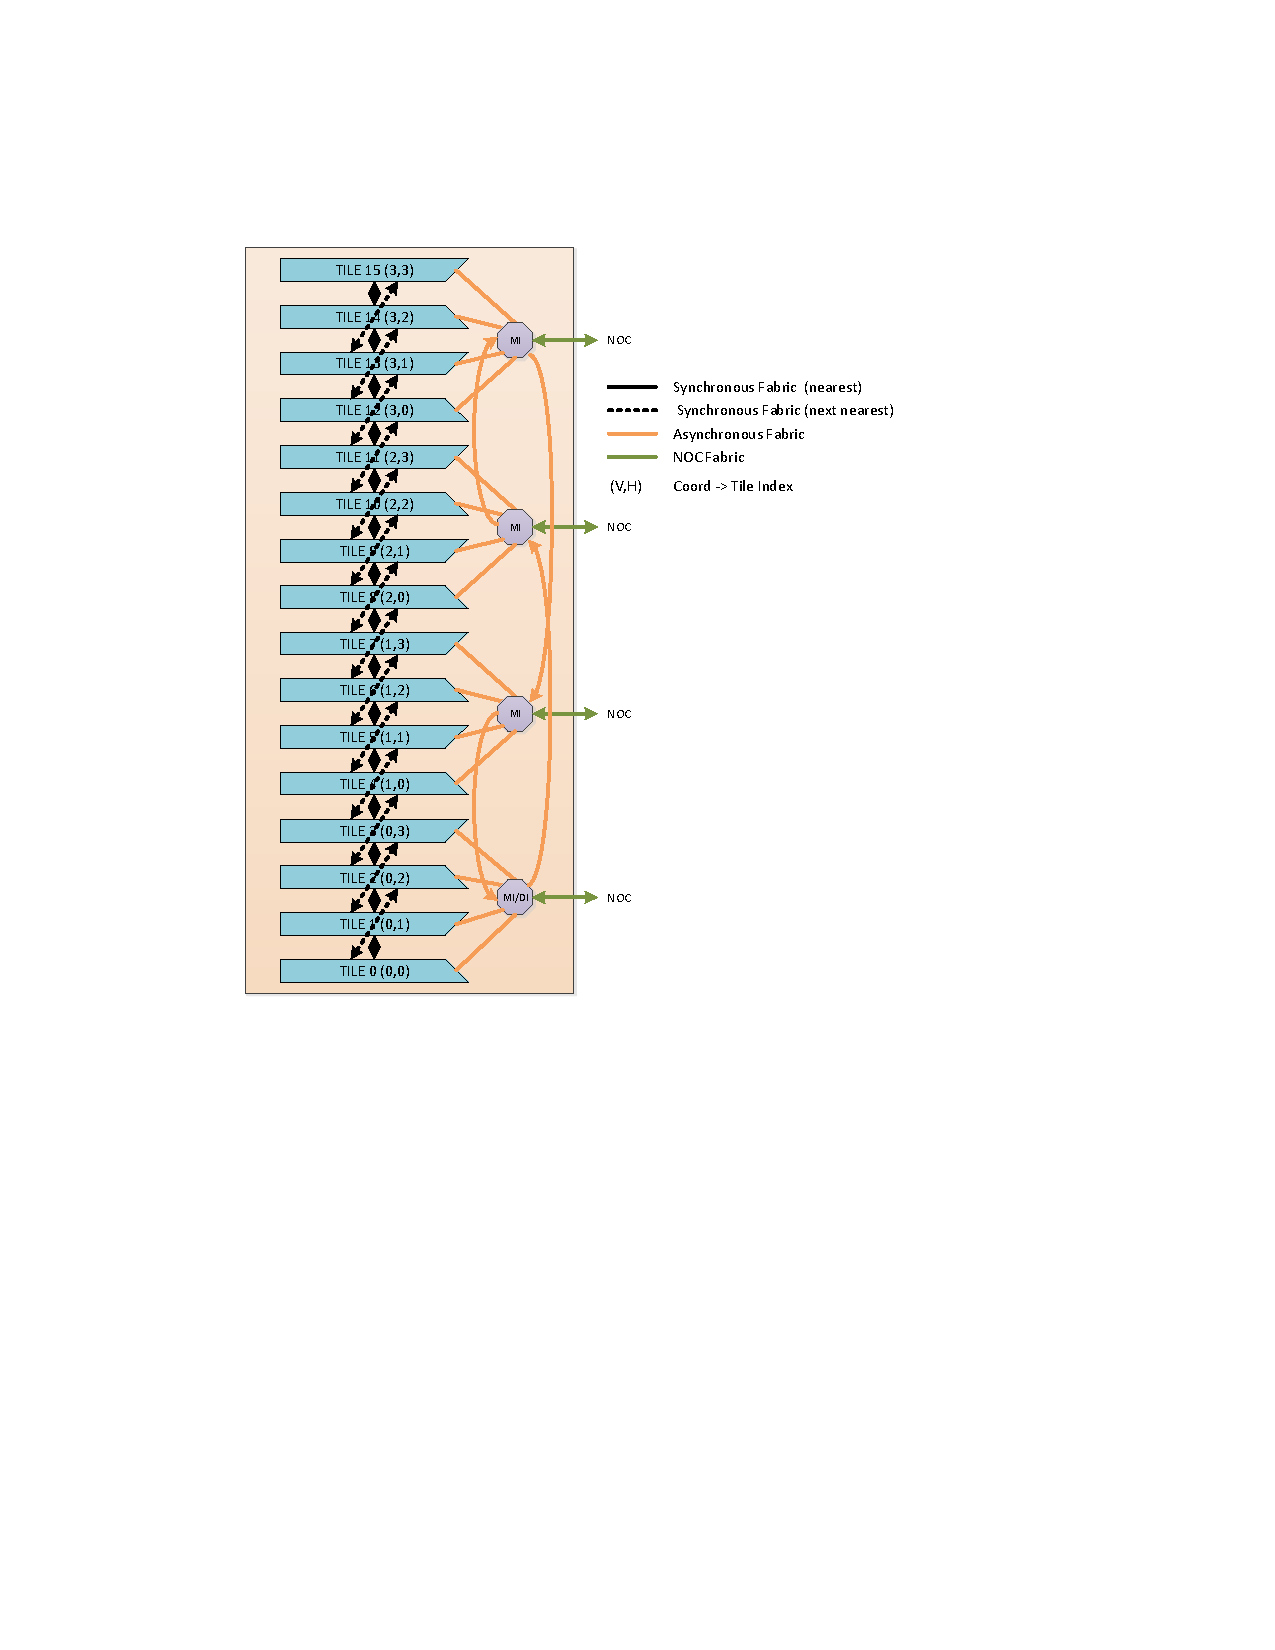
\includegraphics[trim=118 310 180 110, clip, width=\linewidth]{fig/se_device.pdf}
%   % \subfloat[SE tile]{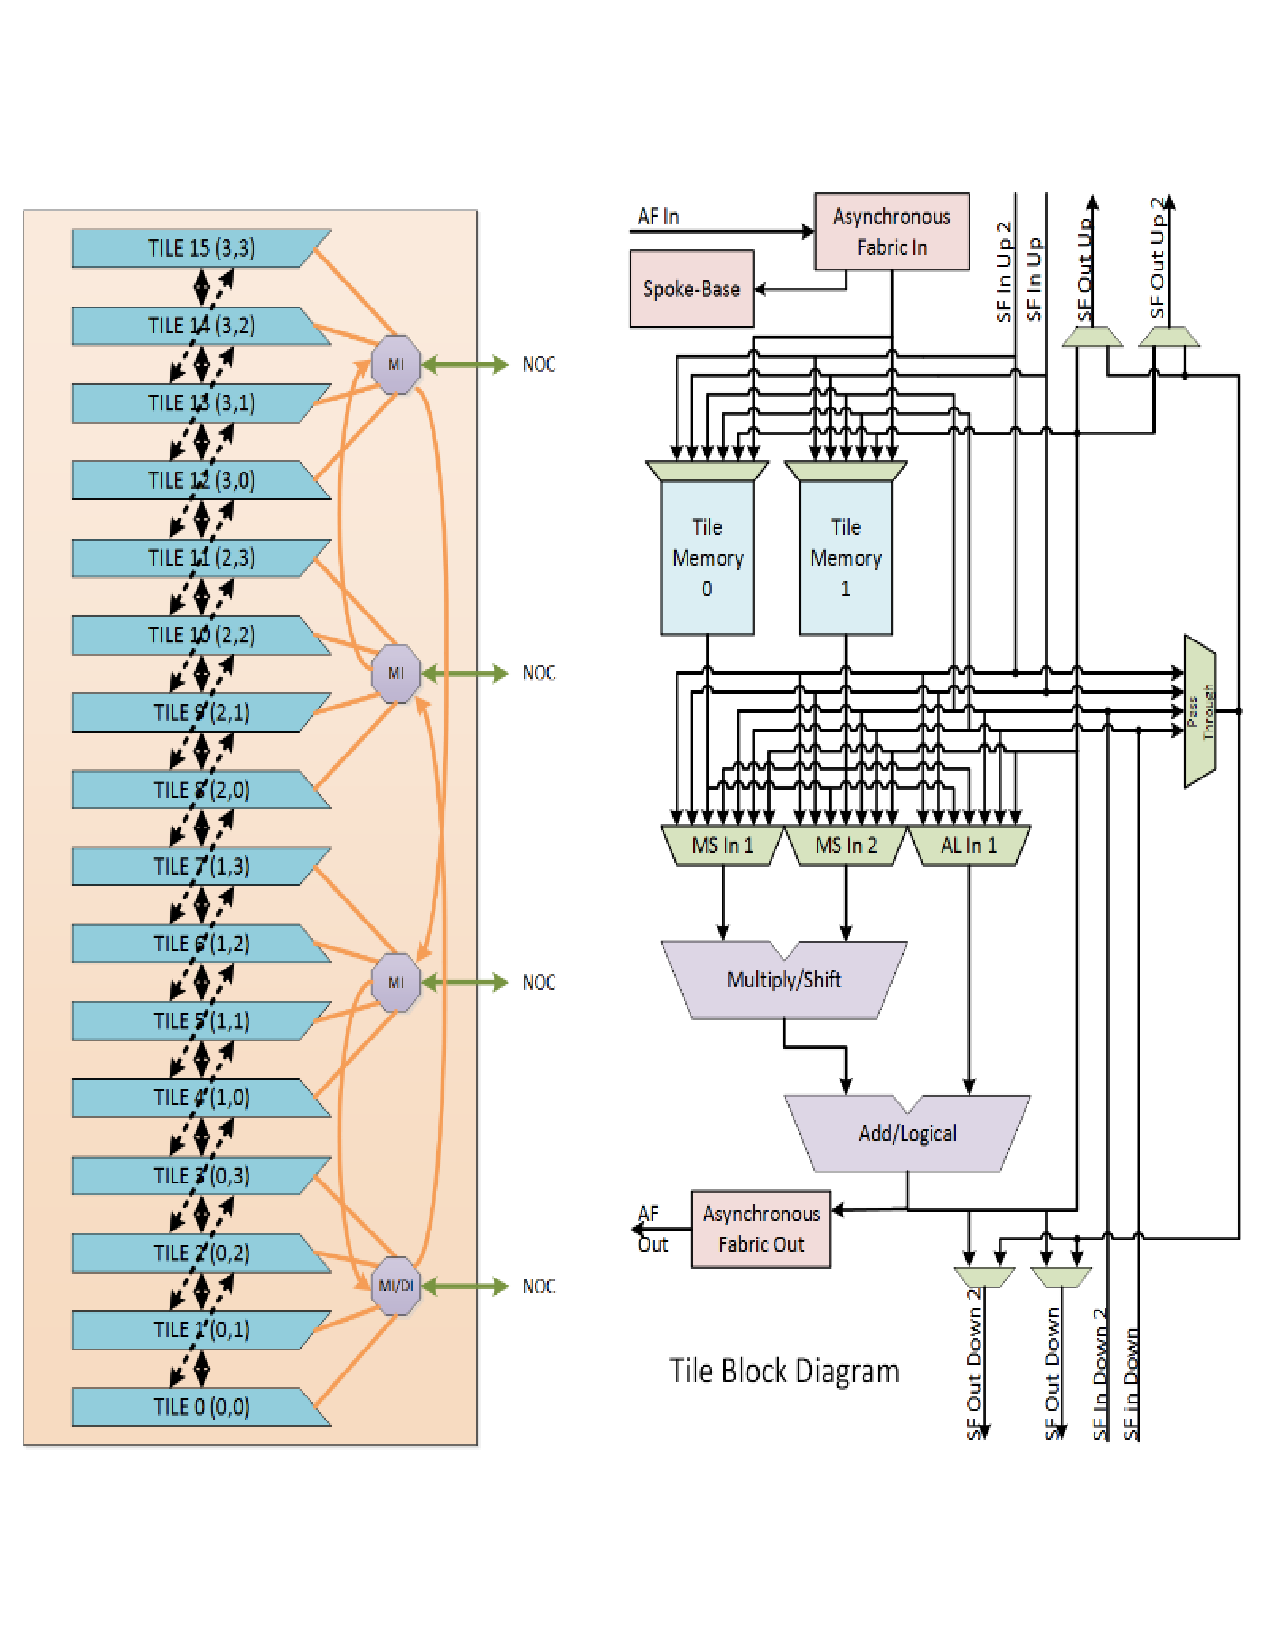
\includegraphics[trim=300 100 8 50, clip, width=0.48\linewidth]{fig/se_device_tile.pdf}}\label{fig:sub-tile}
%   \caption{The layout of the SE device and dataflow paths between tiles.
%   tiles are interconnected in a $1 \times 16$ configuration.
%   }
%   \label{fig:se_diagram}
% \end{figure}

%As shown in the \figurename~\ref{fig:se_diagram}, tiles are interconnected in a $1 \times 16$ configuration.
%The SF is used to connect a tile to another tile one hop above it, a tile two hops above it, a tile one hop below it and a tile two hops below it.
%Information is transferred over the SF with a deterministic latency. 
%Each tile acts independently, streaming data through internal memory and MS/AL units to other tiles over the SF and AF.
%The tiles use the AF to communicate between synchronous domains, send loads and stores to memory through the MI, and receive commands from the host through the DI to initiate work on the SE.
%Information is transferred over the AF with a non-deterministic latency.

% \subsection{Synchronous Fabric Interface}
% All tiles that participate in a synchronous domain act as a single pipelined data path.
% The SDF's entry tile is defined as the tile that executes the first instruction of the SDF.
% It is responsible for initiating a thread of work through the pipelined tiles at a predefined cadence, referred to as the Spoke Count or II.
% E.g., For $II = 3$, as in the example in \figurename~\ref{fig:se_example}, then the entry tile can initiate work every third clock cycle.
% %The synchronous fabric provides both data and control information.

% \subsection{Asynchronous Fabric interface}
% The Asynchronous Fabric is used to perform operations that occur asynchronously to a synchronous domain.
% Each tile contains an interface to the AF.
% AF messages can be classified as either data messages or control.
% Data messages contain a SIMD width data value that is written to one of the two tile memories.
% Control messages are for controlling thread creation, freeing resources, or issuing external memory requests.

% \subsection{Tile Base}
% The tile base contains data structures that are used to initiate an SDF.
% %It receives messages from the SF interface to configure state and set up the necessary conditions to start a synchronous flow.
% %It initiates a flow into the SF when the required conditions are met.
% %It also contains control logic to manage iterations of loops.
% If the tile was an entry tile of an SDF, then the tile base launches a new thread every II.
% The II allows the base logic to launch new threads or continue previously launched threads when all resources needed for execution are available.

% \subsection{Tile Memory}
% Each tile contains two memories.
% Each are the width of the data path (512-bits), and the depth will be in the range of 512 to 1024 elements.
% The tile memories are used to store data required to support data path operations.
% The stored data can be constants loaded as part of the program's arguments, or variables calculated as part of the data flow.
% The tile memory can be written from the AF as either a data transfer from another SDF, or the result of a load operation initiated by another SDF.
% %The tile memory is only read via synchronous data path instruction execution.

% \subsection{Instructions RAM}
% Each tile has an instruction RAM has multiple entries to allow a tile to be time sliced, performing multiple, different operations in a pipelined synchronous domain.
% %Additionally, each time slice could conditionally perform different instructions depending on previous tile time slice data dependent conditional operations. 

% \subsection{Spoke RAM}
% The Spoke RAM has multiple entries to reconfigure the tile at each time slice (clock cycle).
% The number of active spoke RAM slots in a tile is equal to the II of that tile.
% A couple of relevant configurations are: 

% \begin{itemize}
%   \item Which of the four SF inputs, feedback from the output of the tile's MS/AL unit, or the tile base is the master input.
%   \item Which of the four SF outputs are used to send the output of the MS/AL unit to another tile or tiles using SF.
% \end{itemize}

% The Spoke RAM iterates over its slots using a counter that modulo counts from zero to II minus one and back to zero.
% %Using different spoke counts on different tiles can be a powerful mechanism that allows the number of slices required by an inner loop to determine the performance of an application.
% The proposed RL mapper provides the II and the configuration of each spoke RAM slot, including which tile instruction will be active, on each utilized tile.

% \subsection{Programming the SE}
The SE programmer breaks down the desired application into a set of one or more SDFs.
%An SDF is marked by instructions sending and receiving data in deterministic latency.
%All operations with nondeterministic latencies, e.g., load/store requests to the MI, mark either the beginning and/or ending of an SDF.
We have written an in-house parser that enables the programmer to express the program in terms of SDFs using our defined assembly language.
The parser produces an Intermediate Representation (IR) that is used as an input to our proposed mapper.
The IR is a graph representation of the program which consists of SDF subgraphs. 
%Each SDF is a disconnected component of the IR graph. 
%Here every instruction is a node.
Each node represents an instruction that needs to be placed onto a SE tile at the proper time-slice such that when all nodes are placed, the program executes correctly. 
%In \figurename~\ref{fig:se_example}, the edges of the graph represent the data dependencies of the instructions. 
The nodes also contain information about the variables that need to be present in tile memories during instruction execution. 
%The instruction intended to execute at a specific time-slice will only execute when the master input configured at that specific time slot receives a valid control message.
%The tiles can pass data to their neighbors and each tile can be configured with a different number of initiation intervals (II). 
%Each II can be allocated to run a single instruction during program execution. 
%After one cycle, the tiles will move on to the next II, with execution returning to first II after the last. 
%All tiles run the instruction in the same II in parallel. 
%Thus, whenever possible, independent instructions should be mapped to different tiles and same II to exploit parallelism. 
%The first operation of each disconnected component of the computation graph (one component representing a synchronous flow) needs to be placed on different tiles. 

% \paragraph*{SE Mapping Constraints}
The SE hardware imposes constraints that the RL mapper must adhere to in order to for it to produce a valid mapping. These constraints are:
\begin{enumerate}
  \item Instructions that share one or more tile memory variables must be placed on the same tile.
  \item No two or more instructions that start an SDF can share a tile.
  \item No two or more instructions that are siblings in the SDF can share a tile.
\end{enumerate}
The SE device configuration and its constraints are modeled in a simulation environment and a reward function is used to determine the quality of placements obtained.
%To enforce these constraints, we explore two methods in Section \ref{subsec:output_masking}.
%The first method is to give a negative reward when a constraint is violated and the second is creation of a mask on the invalid actions so that the network only outputs valid actions.
%In both cases, placing instructions sub-optimally leads to a reduced reward whereas placements that optimally reduce total execution time of the graph are rewarded. 

\section{Method}
\label{sec:rlmapper}
\subsection{Reinforcement learning}

We present a Reinforcement learning (RL) based framework to explore and optimize the mapping of instructions for a given computation graph to the SE, guided by a reward function that informs the mapping algorithm about the quality of the produced mappings at each step. In this section, we give an overview of the methods used along with the formulation required for detailed description of the various components of the RL approach.

\subsection{Overview}
Proximal Policy Optimization (PPO) \cite{schulman2017proximal} is an RL method that is  widely used for continuous and discrete action problems. 
It trains an actor and a critic model (represented as neural networks).
The actor model is trained to produce actions (node placements in our case) from sample states obtained during simulation and the critic model is trained to match the sampled rewards from the actions produced by the actor using a surrogate loss function. 
This sample and train process is repeated over various iterations. 
In this manner, the problem search space is explored using the reward function as a heuristic.
Our SE mapping task is formulated as a discrete action problem where the goal is to place one node at each time step. 
Samples of SE state, actions performed and rewards obtained at each time step are collected after executing the actions provided by the actor model in simulation. 
These samples are stored in a buffer and are used as data to train the models.
Figure \ref{fig:ppo} shows the overall RL framework. 

The key components of our RL method are as follows:
\begin{itemize}
  \item States: The state is represented by a concatenation of an array of features of placed nodes, a selected node to be placed next and an embedding of the whole computation graph. 
  \item Action: The action consists of the node to be placed along with the tile and spoke location it is to be placed at.
  \item Reward function: The reward obtained is based on the number of clock cycles taken for a node to finish executing after its predecessors finished executing.
  \item Transition function: The transition function gives the probability distribution over next states given the current state and the action to be performed.
\end{itemize}

\begin{figure}[h]
  \centering
  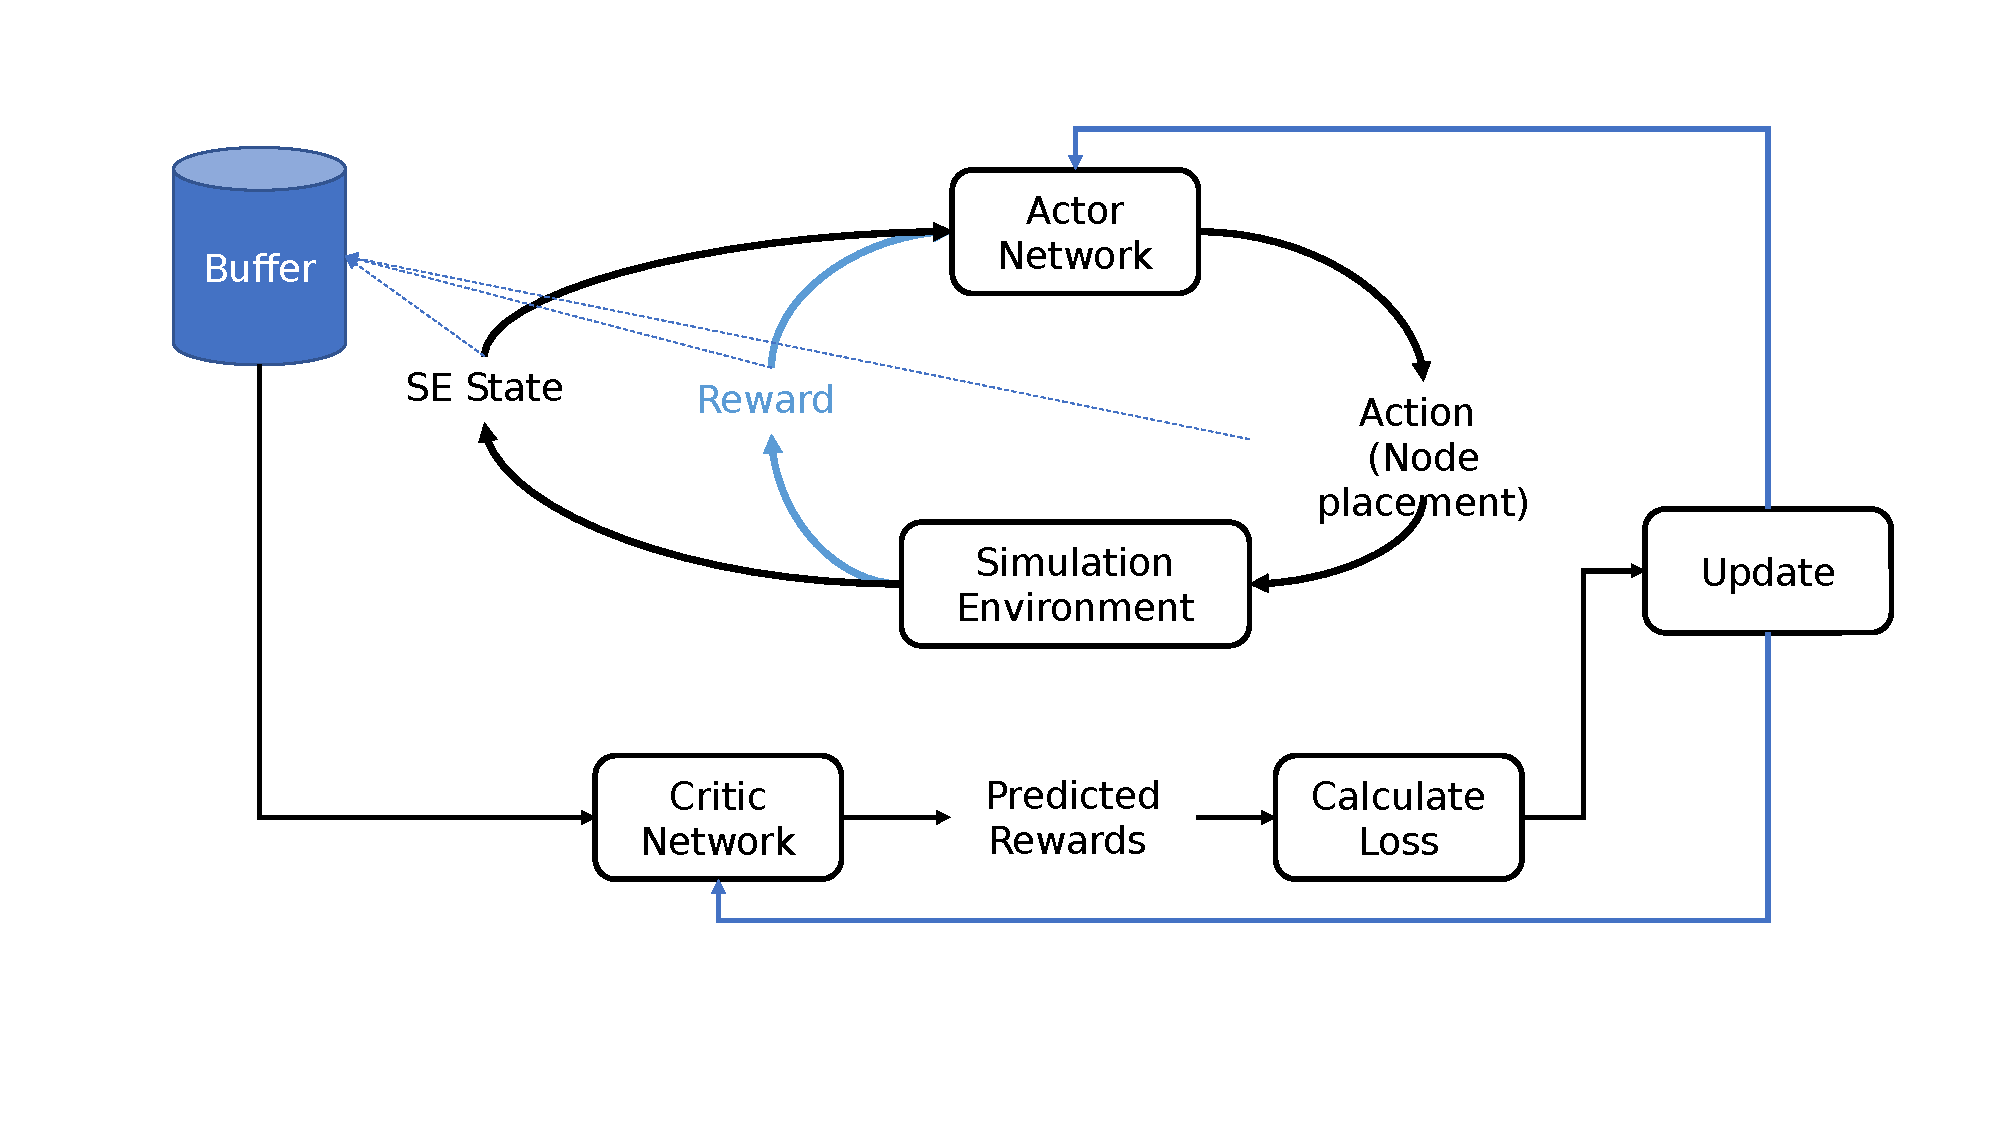
\includegraphics[width=\linewidth]{fig/ppo.pdf}
  \caption{Diagram of the RL framework showing the role of actor and critic networks during RL training. }
  \label{fig:ppo}
\end{figure}

\subsection{State Representation}
The state is a vector of size $|TS|+1$ where $TS$ is the set of tile slices in the Streaming Engine with $TS=T \times I$. Here $T$ and $I$ are sets of all tiles and initiation intervals in the SE respectively.

\subsection{Action Representation}
\todo[inline]{Ensure mathematical notations are consistent throughout paper}
The action at each step is a tuple \((n,t,i)\) where $n \in N$ (the set of all nodes) is the node to be placed and $t \in T$ and $i \in I$ are the tile and initiation interval at which the node $n$ is to be placed. 
We place nodes in a topological order which ensures that all of a node's predecessors have been placed before the node. 
We do not make selecting the node to be placed a part of the learning problem since it increases the complexity of the learning process and makes training harder.

\subsubsection{Masked Actions}
In order to enure that the network only outputs valid actions, we determine a binary mask over all possible actions and set the value of logits corresponding to invalid actions to $-\infty$ in the actor network. 
This in turn sets the probability of sampling invalid actions to $0$, ensuring that we never take an invalid action.
Finally, we only calculate entropy on valid actions, so that our algorithm maximizes exploration only on valid actions.

\subsection{Reward Function}
Our goal in this work is to get mappings that are optimal in terms of total clock cycles taken and for this purpose, the reward that is given at each time step is the difference between the clock cycle at which the current node to be placed is ready (its ready time) and the ready time of its predecessor. 
$R_n$ is the reward obtained for placing node $n$ and $t_n$ is its ready time. 
The function $p(n)$ gives the predecessor of $n$ in a computation graph. 
If the current node can't be placed because of the constraints (all values in the mask vector $m$ are zero), then a high negative reward $-\lambda$ is given.
\[
  R_n =
  \begin{cases}
    -\lambda,& m_i = 0, \, \forall \, i \in T \times I \\
    t_n - t_{p(n)}, & \text{otherwise}
    
  \end{cases}
\]

\subsection{Model design}

The actor and critic models architecture is shown in figure \ref{fig:model}. 
The input is separated in two categories: static and dynamic data. 
Static data is information that doesn't change as nodes are being placed, such as: computation graph and tile memory constraint.
Device state, node to be placed and placed node latencies are dynamic data that changes during placement.

Tile memory variables need to be placed in a tile so that operation can use that variable. 
This memory constraint is captured as memory dependency array. 
Tile memory constraints are incorporated into nodes in the computation graph. 
The computation graph has each node representing an instruction. 
The node features are tile memory dependencies. 
A Graph Neural Network (GNN) is used to process node dependencies and create an embedding for each node. 
An attention module is applied to the embedding matrix to select which dependency nodes are relevant to the current node to be placed. The dynamic data is fed into a MLP model to 
create another embedding to represent current state. 
The two embeddings are combined and fed into another MLP model to 
create actions. 
Invalid actions are masked before being sent to the reward function. Masking was shown to be effective in RL setting \cite{Shengyi_mask}.

\begin{figure*}[h]
  \centering
  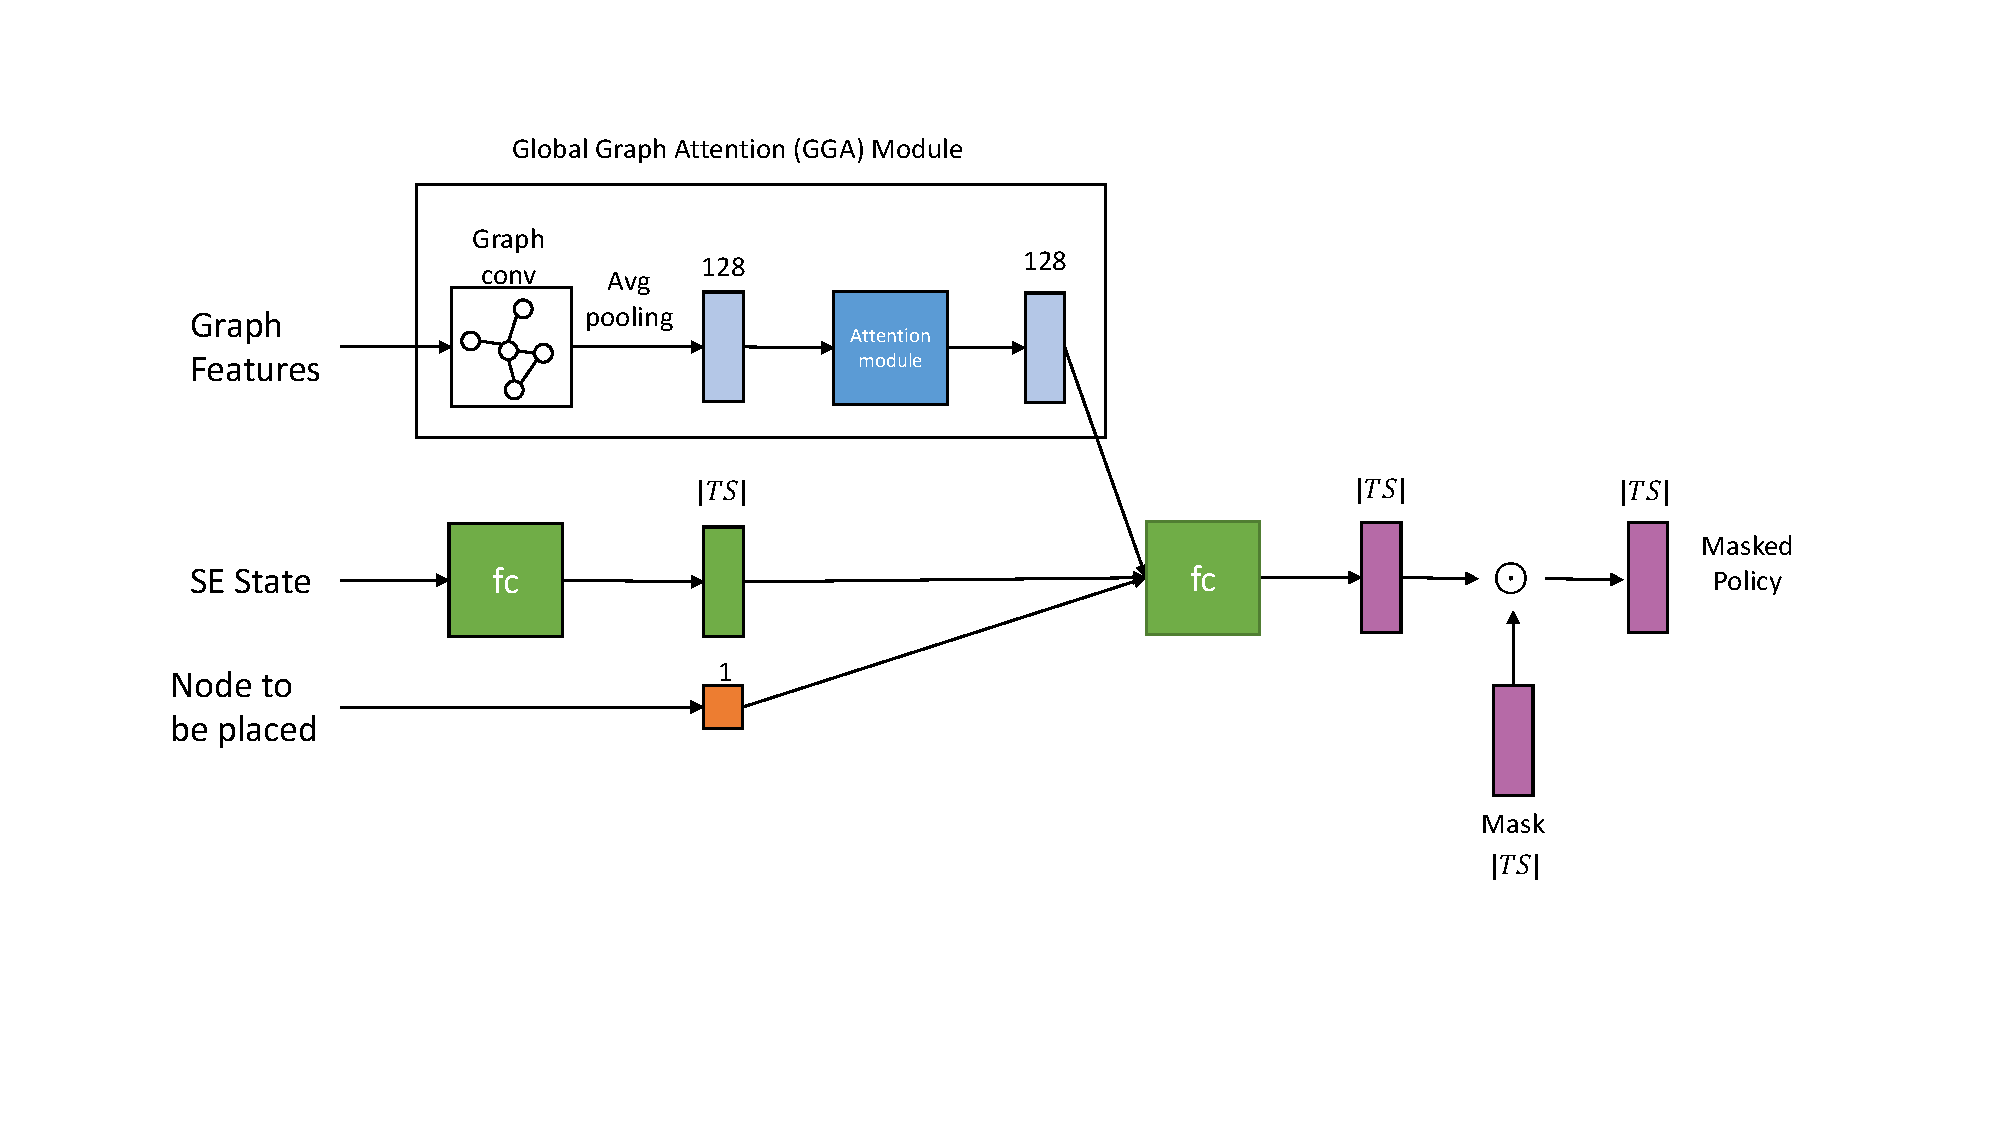
\includegraphics[width=\textwidth]{fig/model_diagram.pdf}
  \caption{Actor and critic model architecture. GNN is used to process the computation graph (static data). 
  Attention module gives importance to relevant nodes. The embedding created from dynamic data is combined with static data embedding. 
  A final MLP model is used to generate actions. Actions are masked to ensure only valid actions are produced. }
  \label{fig:model}
\end{figure*}



\section{Results}
\label{sec:results}
The implemented RL approach was able to successfully map the computation graphs for different programs such as vector add, distance calculation function and IFFT. 
IFFT is widely used by several algorithms and its computation graph is shown in Fig. \ref{fig:ifft_graph} 
The SE device configuration for the following experiments used 16 tiles and a maximum of 6 Initiation Interval (II).
Other SE device configurations could have been used.

\begin{figure}[h]
  \centering
  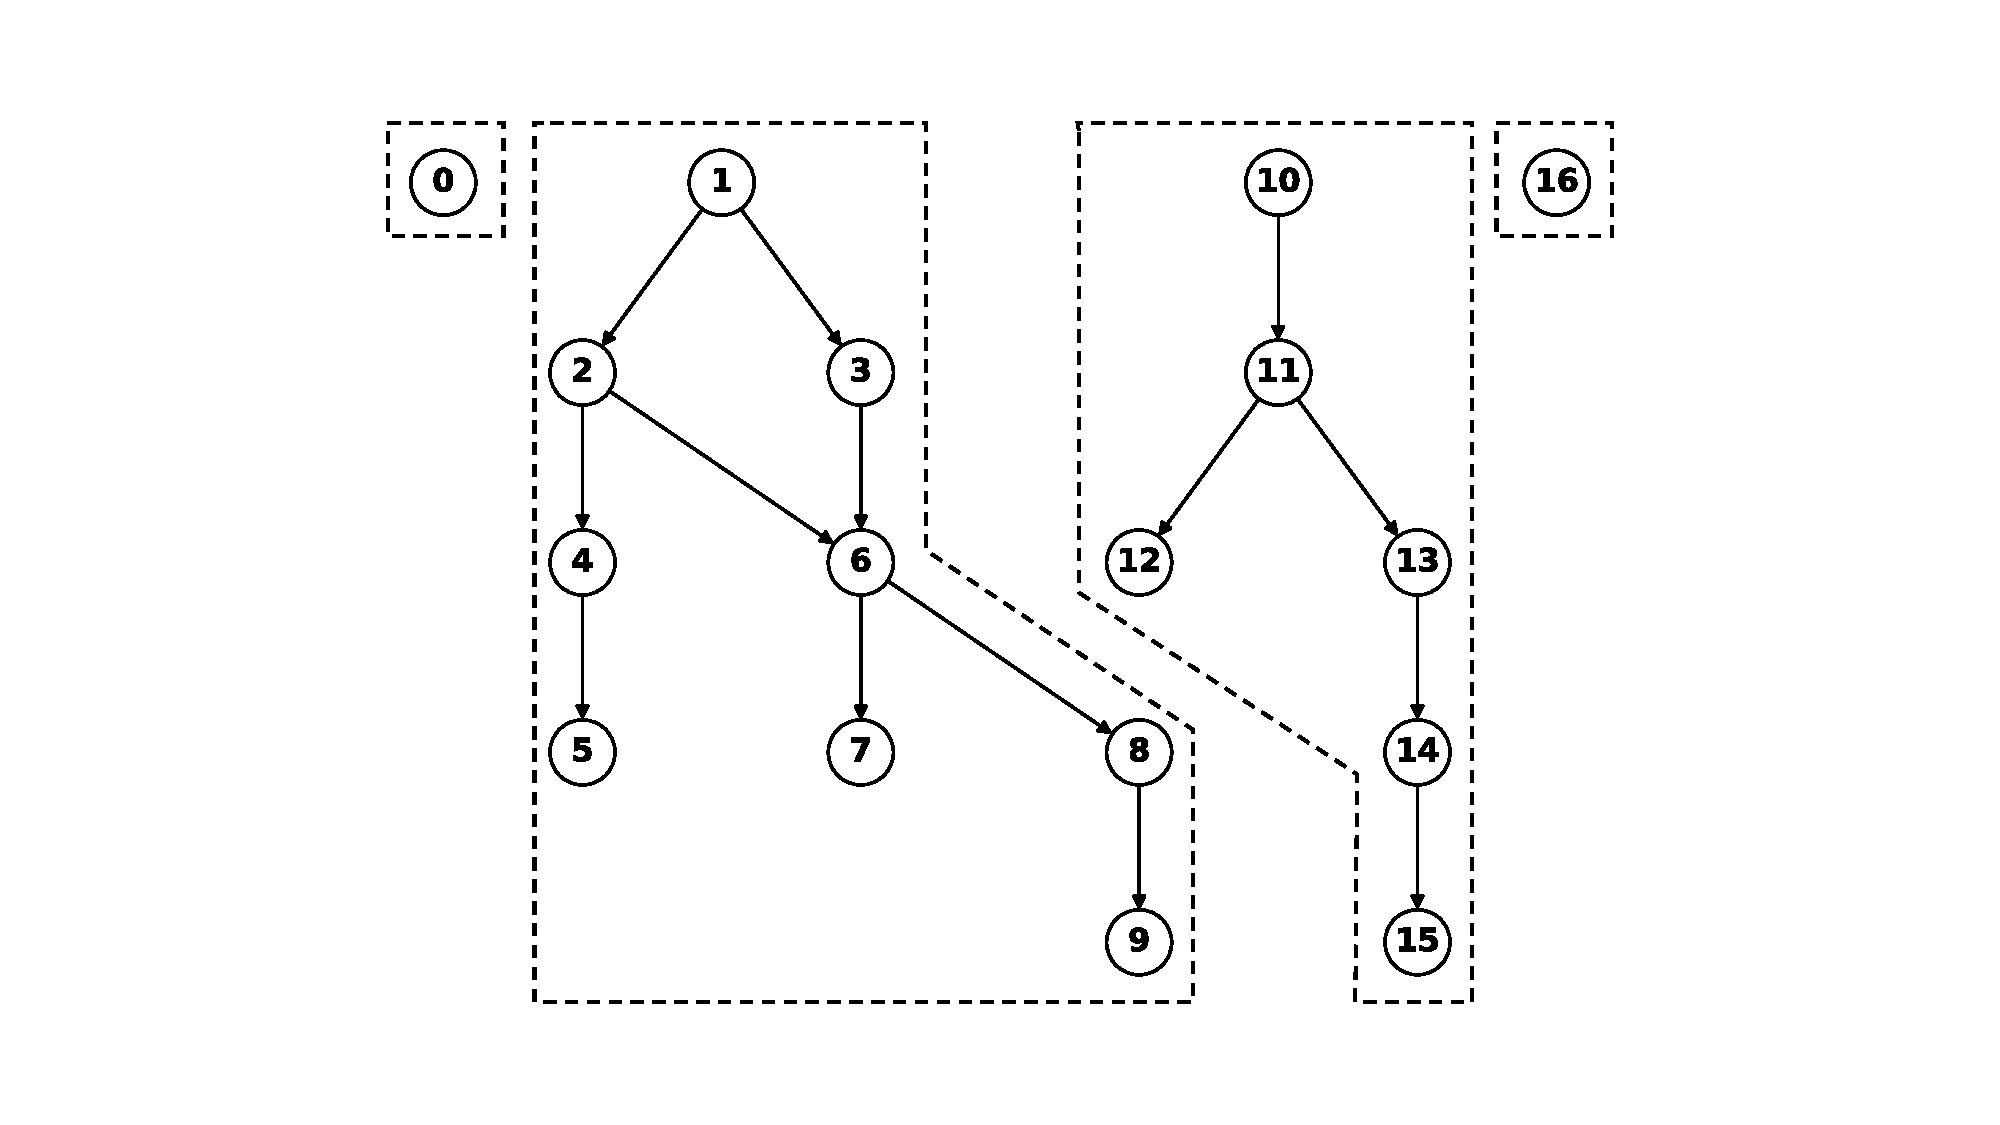
\includegraphics[scale=0.4]{fig/ifft_graph.pdf}
  \caption{IFFT application computation graph.}
  \label{fig:ifft_graph}
\end{figure}


We also benchmarked our RL framework against a collection of random directed graphs. 
We compare a baseline PPO method composed of 3 stacked MLPs against an actor model with the proposed Global Graph Attention (GGA) module.
We evaluate these models on varying computation graphs with different complexities by increasing number of nodes in the graph. 
We also tested on a larger device with 64 tiles.
In Fig. \ref{fig:nodes_graph}, we observe that the RL approach finds mappings for a variety of computation graphs, and GGA
improves the best schedule found for the same number of epochs. The GGA also finds improved schedule for a larger device configuration. 
In the figure \ref{fig:nodes_graph}, the epochs were limited to 50000 for both models. 
The cycle count is number of SE execution steps taken to process all nodes for a mapping, which is calculated from the simulated SE environment. 

\begin{figure}[h]
  \centering
  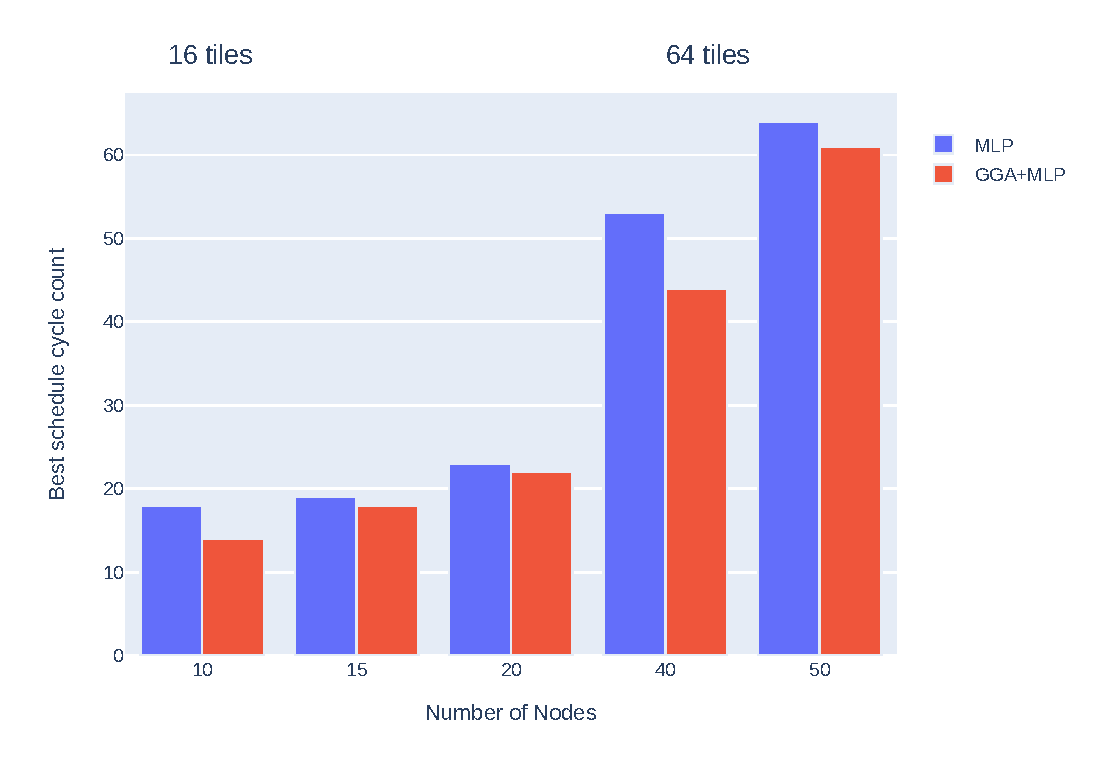
\includegraphics[width=\linewidth]{fig/nodes_graph.pdf}
  \caption{Cycle count for running all nodes in the best mapping given by RL model over 50000 epochs. 
  PPO baseline MLP model and GGA model were evaluated with computation graphs with increasing number of nodes. 
  A larger device configuration with 64 tiles was used for experiments with computation graphs with 40 and 50 nodes. }
  \label{fig:nodes_graph}
\end{figure}


\subsection{Global Graph Attention (GGA)}

In Fig. \ref{fig:ifft_rewards}, we see the addition of GGA module provides improved reward and sample efficiency for the IFFT application. 
The node and states changes for each iteration over all nodes in the computation graph. The GGA module provides a representation of the entire graph while placing each node.

\begin{figure}[h]
  \centering
  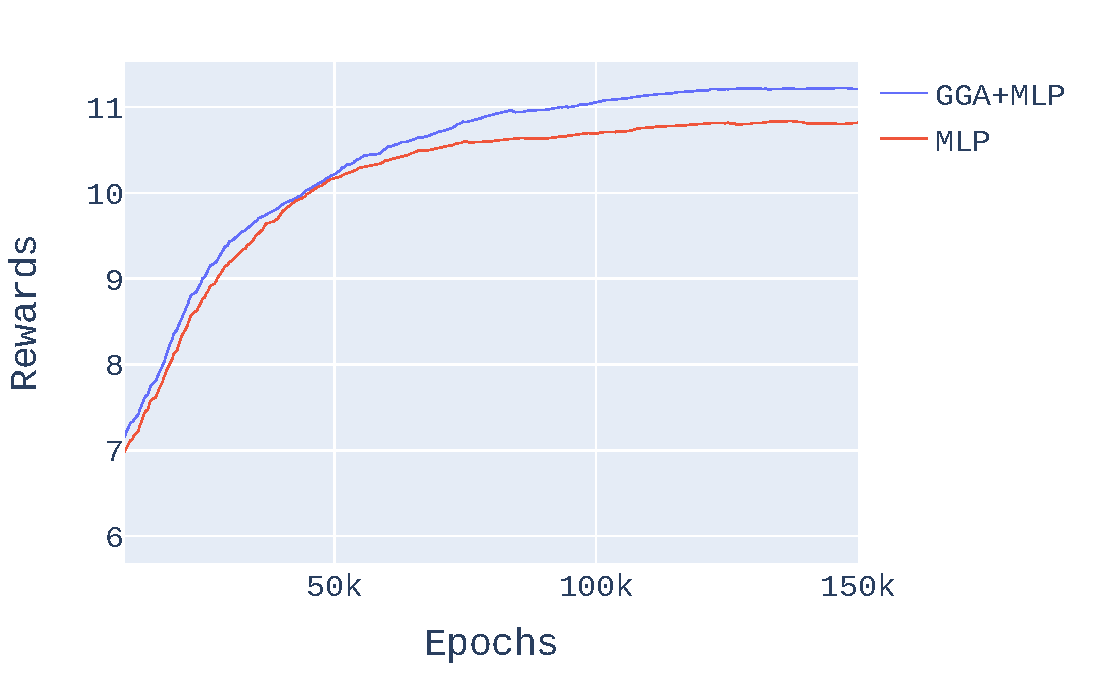
\includegraphics[width=\linewidth]{fig/plot_gnn_atten_ppo.pdf}
  \caption{Effect of using Global Graph Attention (GGA) module for mapping the IFFT application on device with 16 tiles. 
  GGA module provides better sample efficiency and higher reward after training. }
  \label{fig:ifft_rewards}
\end{figure}


\subsection{Node Iteration Order}

The iteration order is sequence in which nodes are fed to the actor model in the RL framework and plays an important role in whether the nodes can be successfully placed or not. 
In Fig. \ref{fig:ordered_placement}, we observe that iterating over nodes in topological 
ordering results in higher reward and eases the node placement task. 
On the other hand, when placing the leaf nodes first, the model needs
to predict which tiles the predecessor nodes will be placed on, making training and the learning problem harder.

\begin{figure}[h]
  \centering
  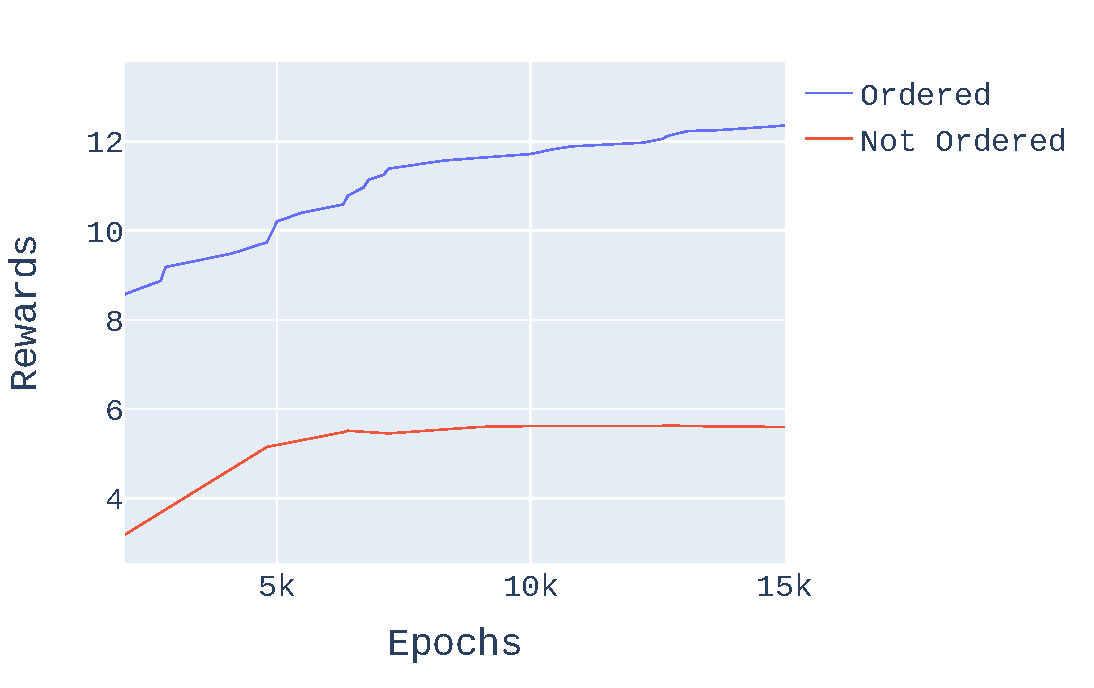
\includegraphics[width=\linewidth]{fig/plot_ordered.pdf}
  \caption{Iterating nodes in topological ordering results in higher reward and eases the placement task. 
 The blue line is the reward curve for when nodes were randomly selected for placement. The red line is the reward curve for when nodes were iterated upon in topological order. The task involved is of placing 15 nodes computation graph in a device with 16 tiles.}
  \label{fig:ordered_placement}
\end{figure}


\subsection{Output Masking}
\label{subsec:output_masking}
Output masking to filter invalid placements has been shown to be effective for RL in game environments \cite{Shengyi_mask}. 
The SE instruction scheduling task has several invalid actions that adds noise to the samples and decision of the RL model, making convergence harder. 
After placement of each node, the following nodes have fewer placement options due to their data dependecy with other nodes and device constraints.
This reduces the search space as each node is being placed. 
Figure \ref{fig:mask_nomask} demonstrates that masking improves the reward and sample efficiency of the RL model.

\begin{figure}[h]
  \centering
  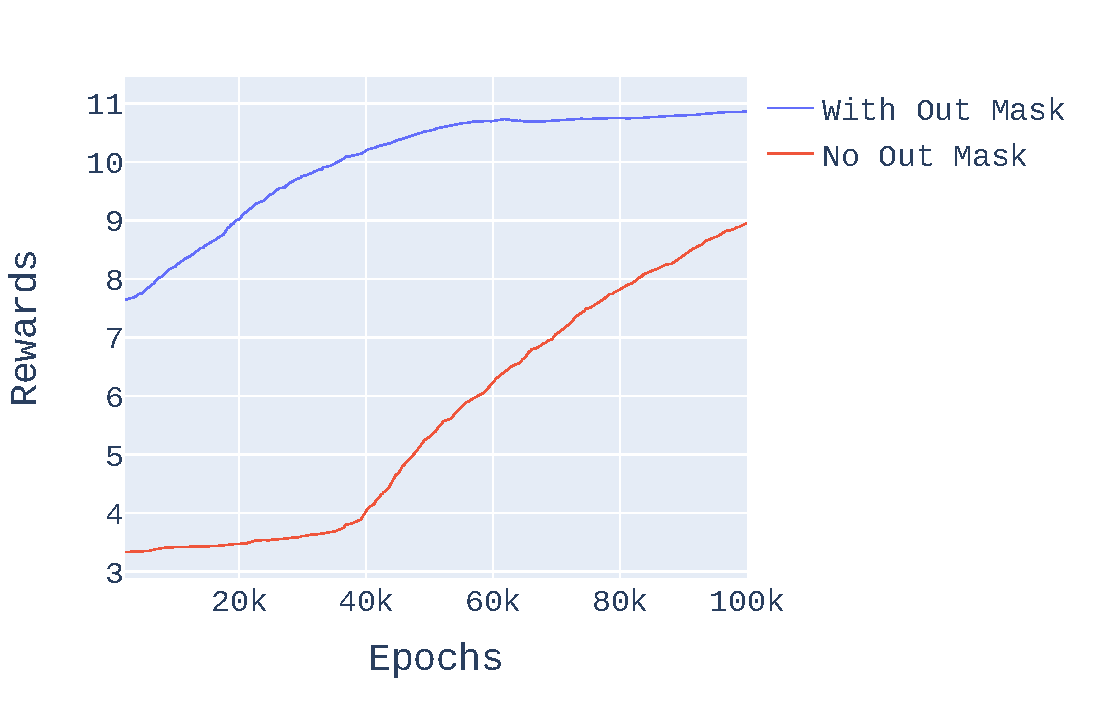
\includegraphics[width=\linewidth]{fig/ifft_masked_nomask.pdf}
  \caption{Reward comparison between node placement with output masking (blue) and without output masking (red).}
  \label{fig:mask_nomask}
\end{figure}


% sequence versus one by one




\section{Conclusion}
\label{sec:conclusion}
Our proposed RL mapper is a key component of the SE device toolchain.
It that enables finding a valid mapping of an application within a reasonable amount of time.
It can search for optimal mappings while using the learning to map previously unseen workloads.
Thus, improving the total time required to get a mapping as compared to the existing manual placement approach and allows for automated search of mappings with different optimizations under different trade-offs, hence reducing the manual labor required to find mappings. 

The chip placement problem space can be modeled as mapping an SDF graph onto a dataflow architecture.
Thus, the presented work has the potential to be applied to chip placement.

Future work includes: 
\begin{itemize}
    \item Optimizing training methods to obtain mappings for problems like FFT which have a bigger search space than currently used SDF graphs. 
    \item Increasing sample efficiency of learning methods and improving the simulation environment for the SE by adding more constraints. 
    \item Studying the impact of reusing the trained networks across graphs rather than training a network from scratch for a given SDF graph.
    \item Integration of RL mapper into the SE toolset.
    \item Investigating the application of the proposed techniques to chip placement problem.
\end{itemize}



%%
%% The acknowledgments section is defined using the "acks" environment
%% (and NOT an unnumbered section). This ensures the proper
%% identification of the section in the article metadata, and the
%% consistent spelling of the heading.
% \begin{acks}

% \end{acks}

%%
%% The next two lines define the bibliography style to be used, and
%% the bibliography file.
\bibliographystyle{ACM-Reference-Format}
\bibliography{sample-base}

%%
%% If your work has an appendix, this is the place to put it.
% \appendix

% \section{Research Methods}

% \subsection{Part One}

% Lorem ipsum dolor sit amet, consectetur adipiscing elit. Morbi
% malesuada, quam in pulvinar varius, metus nunc fermentum urna, id
% sollicitudin purus odio sit amet enim. Aliquam ullamcorper eu ipsum
% vel mollis. Curabitur quis dictum nisl. Phasellus vel semper risus, et
% lacinia dolor. Integer ultricies commodo sem nec semper.

% \subsection{Part Two}

% Etiam commodo feugiat nisl pulvinar pellentesque. Etiam auctor sodales
% ligula, non varius nibh pulvinar semper. Suspendisse nec lectus non
% ipsum convallis congue hendrerit vitae sapien. Donec at laoreet
% eros. Vivamus non purus placerat, scelerisque diam eu, cursus
% ante. Etiam aliquam tortor auctor efficitur mattis.

% \section{Online Resources}

% Nam id fermentum dui. Suspendisse sagittis tortor a nulla mollis, in
% pulvinar ex pretium. Sed interdum orci quis metus euismod, et sagittis
% enim maximus. Vestibulum gravida massa ut felis suscipit
% congue. Quisque mattis elit a risus ultrices commodo venenatis eget
% dui. Etiam sagittis eleifend elementum.

% Nam interdum magna at lectus dignissim, ac dignissim lorem
% rhoncus. Maecenas eu arcu ac neque placerat aliquam. Nunc pulvinar
% massa et mattis lacinia.

\end{document}
\endinput
%%
%% End of file `sample-sigplan.tex'.
